\section{Segmentace objektů pomocí strojového učení}\label{sec:klasifikace-a-segmentace-objektu-pomoci-strojoveho-uceni}

Image segmentation je technika v počítačovém vidění, která má za cíl rozdělit obrázek na několik segmentů nebo oblastí pro jednodušší analýzu.
Cílem image segmentation je identifikovat a rozlišit různé objekty nebo části obrázku, což může být užitečné pro různé aplikace, jako je rozpoznávání objektů, detekce hranic, klasifikace a další analytické úlohy.
V mém případě jsem chtěl využít tuto techniku k tomu, abych identifikoval, která slepice snesla vajíčko, abych tak získal statistiku o tom v jaké kondici slepice jsou a jak dobře snáší.
Existuje několik možností, jak slepici identifikovat, já jsem se rozhodl pro rozpoznání slepice z obrazu.

Nejdříve jsem začal pracovat na získání a přípravě dat.
Shromáždil jsem dataset snímků slepic z kurníku, který pokrývá různé úhly pohledu, osvětlení a pozice.
Dataset jsem anotoval.
V tomto případě byla tvorba anotačního souboru významně složitější, protože bylo třeba nejenom identifikovat, že slepice je na obraze, ale identifikovat její konkrérní tvar, případně jenom část těla.
Znamenalo to tedy ručně projít jednotlivé snímky a myší vyklikat potřebné oblasti, což je znázorněno na obrázku~\ref{fig:label_segmentation}.

\begin{figure}[h]
    \centering
    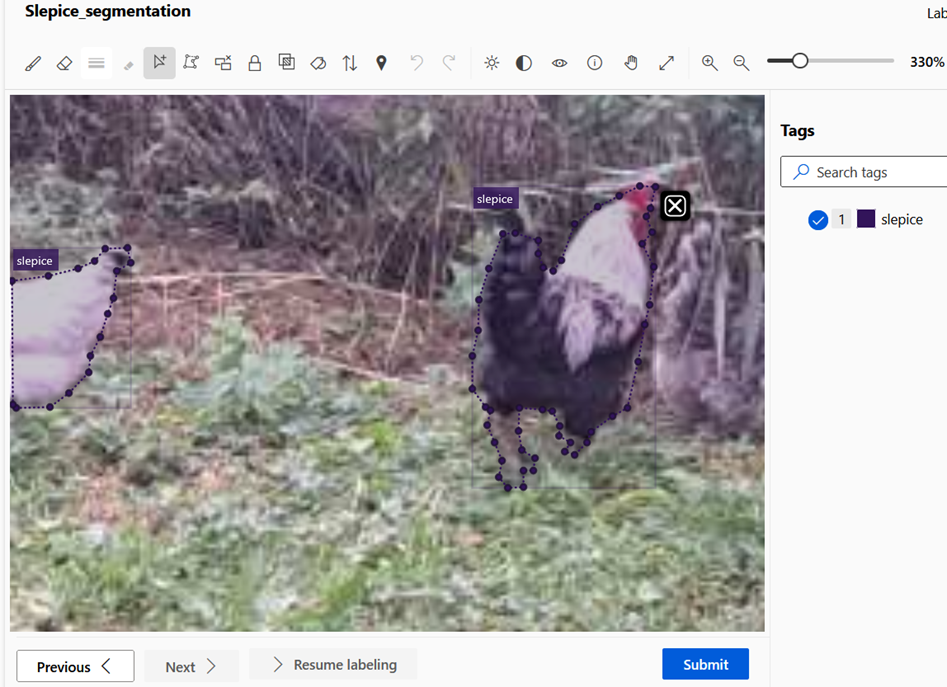
\includegraphics[width=0.8\textwidth]{img/label_segmentation}
    \caption{Proces tvorby metadat pro trénofání segmentace}
    \label{fig:label_segmentation}
\end{figure}

1.	Obecná zásada říká, že platí přímá úměra mezi množstvím trénovacích dat a kvalitou modelu.
Toto jsem mohl vyřešit větším počtem obrázku v testovacím datasetu nebo použít techniku augmentace dat.
To je postup, který jsem zvolil já. Na obrázky jsem aplikoval řadu transformací, které přispěly k různorodosti dat.\newline
\newline
Rotace - otáčení obrázků o náhodně vybrané úhly, aby se model stal invariantním vůči natočení objektů.\newline
Škálování - změny velikosti obrázků buď zmenšením nebo zvětšením, aniž by se změnil poměr stran, což pomáhá modelu lépe zvládat objekty různých velikostí.\newline
Oříznutí (cropping) - vyříznutí náhodných částí obrázku. \newline
To pomáhá modelu naučit se, že objekty mohou být částečně oříznuty.\newline
Překlopení (flipping) - horizontální nebo vertikální zrcadlení obrázku pro zvýšení variability dat.\newline
Změna jasu, kontrastu a saturace - úprava těchto parametrů dělá model odolnějším vůči různým světelným podmínkám.\newline
Přidání šumu - přidání náhodného šumu do obrázků může pomoci modelu být méně citlivý na zašumění v datech.\newline
Posun (translation) - posunutí obrázku ve vodorovném nebo svislém směru, které pomáhá modelu rozpoznávat objekty při různých umístěních.\newline
Random Erasing - náhodné vymazání malých částí obrázku, které může pomoci vylepšit model proti částečnému zakrývání objektů.\newline
MixUp - směšování dvou obrázků a jejich odpovídajících anotací ke generování nových tréninkových vzorů.\newline
Mosaic Augmentation - kombinování čtyř různých obrázků do jednoho, což rozšiřuje kontext a zvyšuje variabilitu scén.\newline
\newline

Následovalo trénování segmentačního Modelu:
Řešení jsem postavil na YOLO11 z oficiálního repozitáře.
Díky knihovnám z projektu Ultralytics je volání přímočaré.
Na vstup jsem dal cestu k obrázkovému datasetu a anotačnímu souboru v COCO formátu.
Další parametry jsem pro výuku ponechal defaultní.
Počet epoch jsem ponechal na 50.
Již od 40 epochy model dosahoval přijatelné úrovně přesnosti při rozpoznávání a segmentaci slepic.

Výsledek segmentace je vidět na obrázku ~\ref{fig:segmented_chicks}.



\begin{figure}[htbp]
    \centering
    % První řádek
    \begin{minipage}[b]{0.8\textwidth}
        \centering
        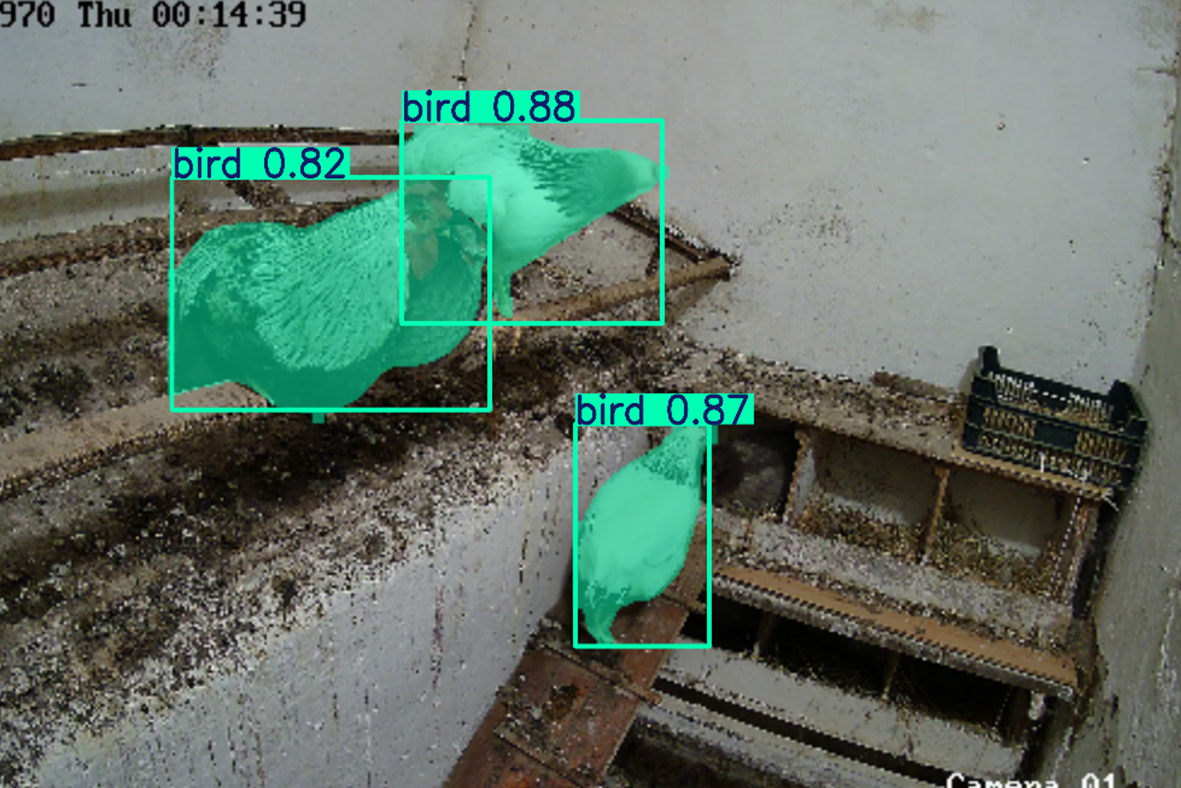
\includegraphics[width=0.8\textwidth]{img/chicken_detection2}
        \caption{Výsledek detekce slepic 1}
        \label{fig:chicken_detection2}
    \end{minipage}

    \vskip\baselineskip % Vertikální mezera mezi řádky

    % Druhý řádek
    \begin{minipage}[b]{0.8\textwidth}
        \centering
        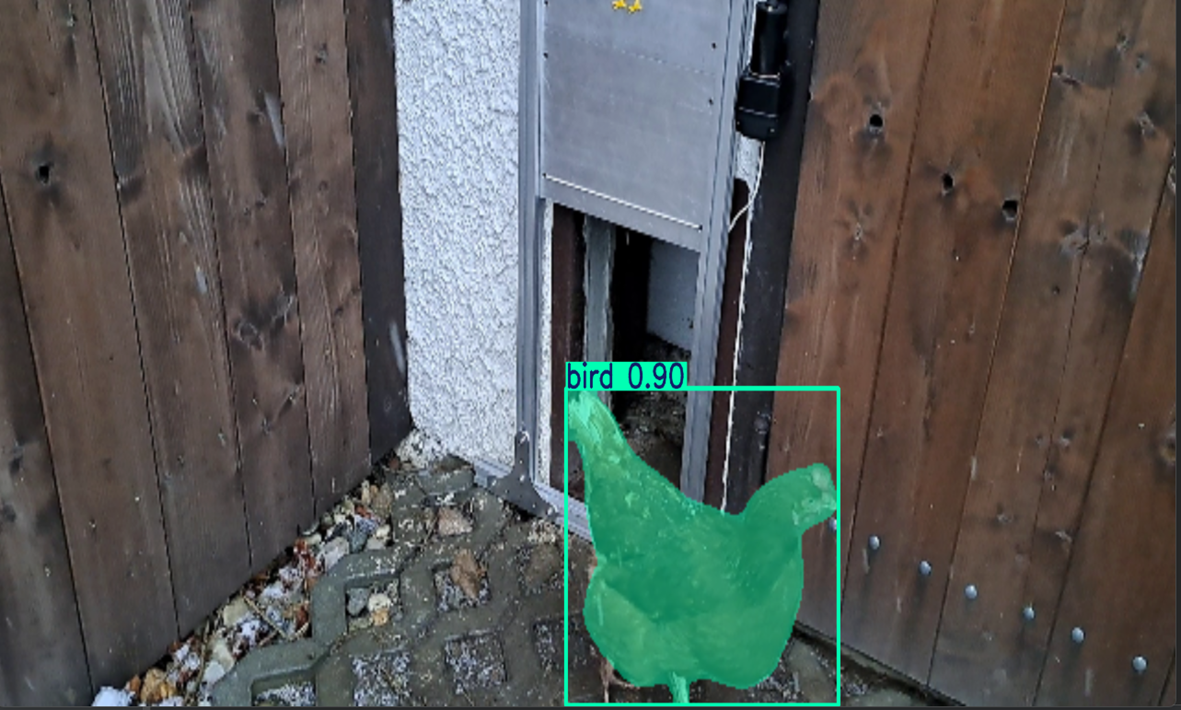
\includegraphics[width=0.8\textwidth]{img/chicken_detection4}
        \caption{Výsledek detekce slepic 2}
        \label{fig:chicken_detection4}
    \end{minipage}
\end{figure}

